\documentclass[a4page,notitlepage]{article}
\usepackage{color,amsmath,graphicx,subcaption,geometry}
\usepackage[citestyle=authoryear]{biblatex}
\usepackage{tikz}
\usepackage{pgfplots}
\usepackage{stackengine,ifthen}
\usetikzlibrary{arrows,positioning,calc}
\newcounter{figstack}
\newcounter{figindex}
\newlength\fight
\newcommand\pushfigure[4][b]{%
  \stepcounter{figstack}%
  \expandafter\def\csname %
    figalign\romannumeral\value{figstack}\endcsname{#1}%
  \expandafter\def\csname %
    figwd\romannumeral\value{figstack}\endcsname{#2}%
  \expandafter\def\csname %
    figcontent\romannumeral\value{figstack}\endcsname{#3}%
  \expandafter\def\csname %
    figcap\romannumeral\value{figstack}\endcsname{#4}%
  \setbox0 = \hbox{%
    \begin{minipage}{#2}#3\end{minipage}}%
  \ifdim\dimexpr\ht0+\dp0\relax>\fight\global\setlength{\fight}{%
  \dimexpr\ht0+\dp0\relax}\fi%
}

\newcommand\popfigures{%
  \setcounter{figindex}{0}%
  \hfill%
  \whiledo{\value{figindex}<\value{figstack}}{%
    \stepcounter{figindex}%
    \def\tmp{\csname figwd\romannumeral\value{figindex}\endcsname}%
    \begin{minipage}[t]{\tmp}%
      \centering%
      \stackinset{c}{}%
      {\csname figalign\romannumeral\value{figindex}\endcsname}{}%
      {\csname figcontent\romannumeral\value{figindex}\endcsname}%
      {\rule{0pt}{\fight}}\par%
      \csname figcap\romannumeral\value{figindex}\endcsname%
    \end{minipage}%
    \hfill%
  }%
  \setcounter{figstack}{0}%
  \setlength{\fight}{0pt}%
  \hfill%
}

\setlength\abovecaptionskip{6pt}
\providecommand{\abs}[1]{\lvert#1\rvert}
\providecommand{\norm}[1]{\lVert#1\rVert}


\title{Analyzing stability of very simple metabolic cycles}
\author{Uri Barenholz}
\date{August 2013}

\begin{document}
\abstract{
    Auto-catalytic cycles are an important part of metabolic networks.
    As the flux in auto-catalytic cycles both depends on the concentration of intermediate metabolites, and affects it, they present unique features and characteristics.
    An understanding of the constraints under which metabolic auto-catalytic cycles operate is essential for realizing limitations of existing metabolic networks, as well as to successfully modify them in synthetic biology metabolic engineering applications.

    We analyze a simple metabolic auto-catalytic cycle, presenting the mathematical tools and techniques needed in order to gain insights about its operation.
    We show that even for very simple cycles, specific constraints on the kinetic parameters of the enzymes are needed in order to allow a stable flux through the cycle.
    This work thus serves as an approachable introduction to the analysis of auto-catalytic metabolic cycles and to derive specific insights about the cycles we analyze.
}

\section{Introduction}
    Metabolic networks topology and function are limited by numerous constraints.
    Stochiometries must be maintained and reactions must be balanced, reactions sharing the same substrates or products must operate at correct ratios, and the entire metabolic network must be stable under noisy environmental conditions.
    Auto catalytic cycles present specific challenges as their inherent feed-back nature makes them susceptible to divergence or drainage.

    In this work we present the specific requirements auto-catalytic cycles must meet in order to operate: (A) To be able to achieve at least one, non-zero, steady state of fluxes. (B) To be stable for fluctuations at the steady state point(s).
    The mathematical tools we define and use are widely known and applicable in various fields.
    Our analysis demonstrates the use of such tools to gain insights about the operation, limitations, and various modifications available to metabolic auto-catalytic cycles in vivo.
\section{A simple auto-catalytic cycle}
    We consider the simple auto-catalytic cycle depicted in Figure \ref{fig:autocatal}.
    This cycle has a single intermediate metabolite, $X$, one auto-catalytic reaction with flux $f_a$ (implying that for any unit of $X$ consumed, it produces two units of $X$), and one outgoing reaction using the cycle substrate with flux $f_b$.
    We assume simple, irreversible Michaelis-Menten kinetics for the two reactions such that:
    \begin{eqnarray*}
      f_a = \frac{V_{\max,a}X}{K_{m,a}+X} \\
      f_b = \frac{V_{\max,b}X}{K_{m,b}+X}
    \end{eqnarray*}
    where all the kinetic parameters are positive.
    \begin{figure}[h]
        \pushfigure[c]{.3\linewidth}%
        {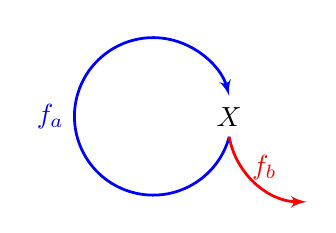
\begin{tikzpicture}[>=latex',node distance = 2cm]
            \node (X) {$X$};
            \draw [->,line width=1pt,blue] (X.south) arc (345:15:1cm) node [pos=0.5,left] {$f_a$};
            \draw [->,line width=1pt,red] (X.south) arc (190:270:1cm) node [pos=0.3,right] {$f_b$};
        \end{tikzpicture}}%
        {\subcaption{Auto-catalytic cycle\label{fig:autocatal}}}
        \pushfigure[c]{.3\linewidth}
        {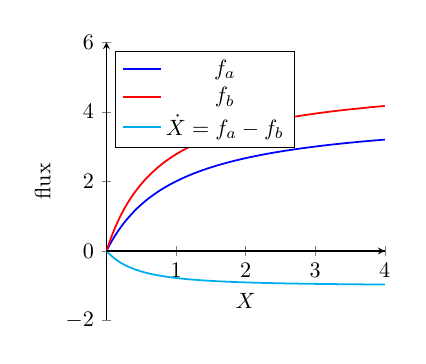
\begin{tikzpicture}[scale=0.8]
            \begin{axis}[axis x line=middle,axis y line=left,xlabel near ticks,ylabel near ticks,xmin=0,ymin=-2,xmax=4,ymax=6,xlabel={$X$},ylabel={flux},legend pos=north west,samples=100,width=6cm,height=6cm]
            \addplot[domain=0:4,blue,thick] {4*x/(1+x)};
            \addplot[domain=0:4,red,thick] {5*x/(0.8+x)};
            \addplot[domain=0:4,cyan,thick] {4*x/(1+x)-5*x/(0.8+x)};
            \addplot[domain=0:4,black,thick] {0};
            \addlegendentry{$f_a$};
            \addlegendentry{$f_b$};
            \addlegendentry{$\dot{X}=f_a-f_b$};
          \end{axis}
        \end{tikzpicture}}
        {\subcaption{Flux response to substrate concentration when $V_{\max,a}<V_{\max,b}$ and $\frac{V_{\max,a}}{K_{m,a}}>\frac{V_{\max,b}}{K_{m,b}}$ \label{fig:michmennointerceptstable}}}
        \pushfigure[c]{.3\linewidth}
        {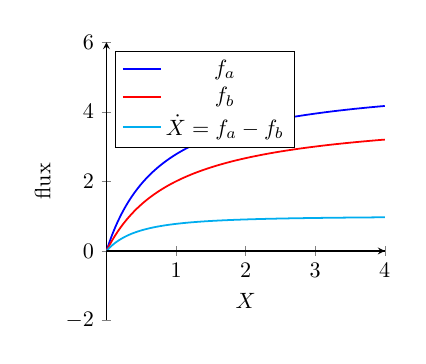
\begin{tikzpicture}[scale=0.8]
            \begin{axis}[axis x line=middle,axis y line=left,xlabel near ticks,ylabel near ticks,xmin=0,ymin=-2,xmax=4,ymax=6,xlabel={$X$},ylabel={flux},legend pos=north west,samples=100,width=6cm,height=6cm]
            \addplot[domain=0:4,blue,thick] {5*x/(0.8+x)};
            \addplot[domain=0:4,red,thick] {4*x/(1+x)};
            \addplot[domain=0:4,cyan,thick] {5*x/(0.8+x)-4*x/(1+x)};
            \addplot[domain=0:4,black,thick] {0};
            \addlegendentry{$f_a$};
            \addlegendentry{$f_b$};
            \addlegendentry{$\dot{X}=f_a-f_b$};
          \end{axis}
        \end{tikzpicture}}
        {\subcaption{Flux response to substrate concentration when $V_{\max,a}>V_{\max,b}$ and $\frac{V_{\max,a}}{K_{m,a}}<\frac{V_{\max,b}}{K_{m,b}}$ \label{fig:michmennointerceptunstable}}}
        \popfigures\par
        \pushfigure[c]{.4\linewidth}
        {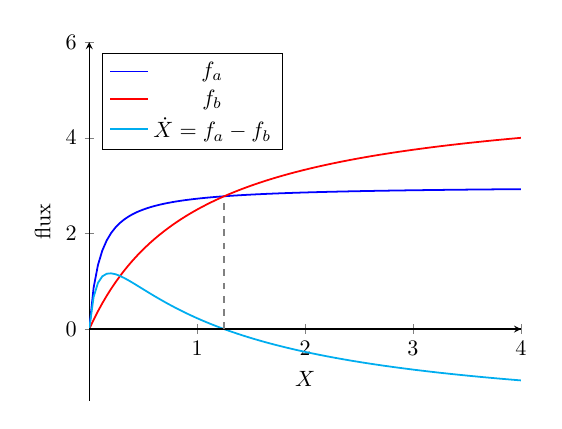
\begin{tikzpicture}[scale=0.8]
            \begin{axis}[axis x line=middle,axis y line=left,xlabel near ticks,ylabel near ticks,xmin=0,ymin=-1.5,xmax=4,ymax=6,xlabel={$X$},ylabel={flux},legend pos=north west,samples=100]
            \addplot[domain=0:4,blue,thick] {3*x/(0.1+x)};
            \addplot[domain=0:4,red,thick] {5*x/(1+x)};
            \addplot[domain=0:4,cyan,thick] {3*x/(0.1+x)-5*x/(1+x)};
            \addplot[domain=0:4,black,thick] {0};
            \addplot[dashed,gray,thick] coordinates {(1.25,0) (1.25,2.77)};
            \addlegendentry{$f_a$};
            \addlegendentry{$f_b$};
            \addlegendentry{$\dot{X}=f_a-f_b$};
          \end{axis}
        \end{tikzpicture}}
        {\subcaption{Flux response to substrate concentration when $V_{\max,a}<V_{\max,b}$ and $\frac{V_{\max,a}}{K_{m,a}}>\frac{V_{\max,b}}{K_{m,b}}$ \label{fig:michmeninterceptstable}}}
        \pushfigure[c]{.4\linewidth}
        {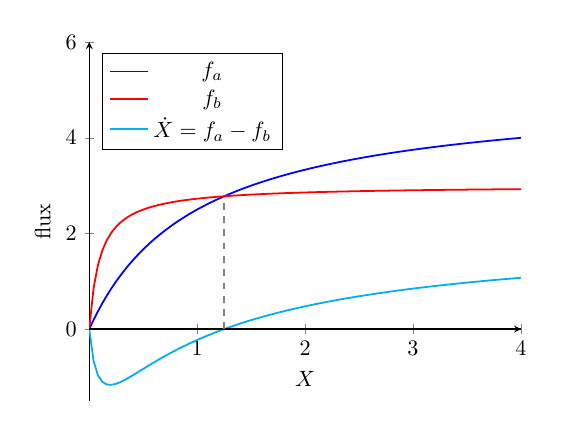
\begin{tikzpicture}[scale=0.8]
            \begin{axis}[axis x line=middle,axis y line=left,xlabel near ticks,ylabel near ticks,xmin=0,ymin=-1.5,xmax=4,ymax=6,xlabel={$X$},ylabel={flux},legend pos=north west,samples=100]
            \addplot[domain=0:4,blue,thick] {5*x/(1+x)};
            \addplot[domain=0:4,red,thick] {3*x/(0.1+x)};
            \addplot[domain=0:4,cyan,thick] {5*x/(1+x)-3*x/(0.1+x)};
            \addplot[domain=0:4,black,thick] {0};
            \addplot[dashed,gray,thick] coordinates {(1.25,0) (1.25,2.77)};
            \addlegendentry{$f_a$};
            \addlegendentry{$f_b$};
            \addlegendentry{$\dot{X}=f_a-f_b$};
          \end{axis}
        \end{tikzpicture}}
        {\subcaption{Flux response to substrate concentration when $V_{\max,a}>V_{\max,b}$ and $\frac{V_{\max,a}}{K_{m,a}}<\frac{V_{\max,b}}{K_{m,b}}$ \label{fig:michmeninterceptunstable}}}
        \popfigures\par

        \caption{A simple auto-catalytic cycle (\subref{fig:autocatal}) induces two fluxes, $f_a$ and $f_b$ as a function of the concentration of $X$.
        A non zero steady state occurs where the fluxes are equal, implying that $\dot{X}=0$ ((\subref{fig:michmeninterceptstable}) and (\subref{fig:michmeninterceptunstable})).
        The steady state is stable if at the steady state point $\frac{d\dot{X}}{dX}<0$ (\subref{fig:michmeninterceptstable}).}
    \end{figure}

    We define the metabolic state of a system by the set of concentrations of all the metabolites in the system.
    In this simple cycle the metabolic state is just the concentration of $X$.
    We note that knowing the concentration of all of the metabolites suffices in order to calculate the fluxes originating from those metabolites, $f_a$ and $f_b$.
    A steady state is defined as a concentration (or set of concentrations) which induces fluxes that keep the concentrations steady, i.e. that the total in-flux to any intermediate metabolite is exactly equal to the total out-flux from that metabolite.
    In our example, a steady state must therefore satisfy:
    \begin{equation*}
      \dot X = \frac{dX}{dt} = 2f_a - f_b - f_a = 0
    \end{equation*}

    Expanding this condition results in getting that:
    \begin{equation*}
      \dot X = 0 \Rightarrow f_a = f_b \Rightarrow \frac{V_{\max,a}X}{K_{m,a}+X}=\frac{V_{\max,b}X}{K_{m,b}+X}
    \end{equation*}
    which is satisfied either if $X=0$ or if:
    \begin{equation*}
      X=\frac{V_{\max,b}K_{m,a}-V_{\max,a}K_{m,b}}{V_{\max,a}-V_{\max,b}}
    \end{equation*}
    As physiologically the concentration of $X$ can only be positive, we get a constraint on the kinetic parameters for which a non-zero steady state may exist.
    This constraint is graphically illustrated in Figures \ref{fig:michmeninterceptstable} and \ref{fig:michmeninterceptunstable}.
    Mathematically the constraint states the sign of $V_{\max,a}-V_{\max,b}$ must be the same as the sign of $V_{\max,b}K_{m,a}-V_{\max,a}K_{m,b}$, implying that the reaction with higher maximal flux must have a shallower slope at $X=0$.

    While having a non-zero concentration steady state is an essential condition to sustain flux, it is not sufficient.
    The non-zero concentration steady state must also be stable to small perturbations.
    Stability with respect to small perturbations is determined by the response of the system to small deviations from the steady state, $X^*$.
    In the single intermediate metabolite case (one dimensional case) stability dictates that at $X=X^*$ it holds that $\frac{d\dot X}{dX} <0$, as this  implies that for points with a small deviation from the steady state: $X = X^*+\Delta X$ the net flux $\dot X$ will oppose the direction of the deviation.
    If $\Delta X$ is positive then $\dot X$ will be negative at $X^*+\Delta X$, reducing $X$ back to $X^*$, and if $\Delta X$ is negative, $\dot X$ will be positive, increasing $X$ back to $X^*$.

    In our case, this condition implies that:
    \begin{equation*}
      \frac{d\dot X}{dX}\Big\vert_{X^*} = \frac{V_{\max,a}K_{m,a}}{(K_{m,a}+X^*)^2}-\frac{V_{\max,b}K_{m,b}}{(K_{m,b}+X^*)^2}<0
    \end{equation*}
    Substituting for $X^*=0$ gives that $0$ is a stable steady state point if $\frac{V_{\max,a}}{K_{m,a}}<\frac{V_{\max,b}}{K_{m,b}}$ and is unstable otherwise.
    For $X^*=\frac{V_{\max,b}K_{m,a}-V_{\max,a}K_{m,b}}{V_{\max,a}-V_{\max,b}}$ we get the opposite condition, i.e. that it is stable if $\frac{V_{\max,a}}{K_{m,a}}>\frac{V_{\max,b}}{K_{m,b}}$ and unstable otherwise.
    
    These results can be intuitively understood with the help of Figures \ref{fig:michmeninterceptstable} and \ref{fig:michmeninterceptunstable}.
    For Michaelis Menten kinetics, $\frac{V_{\max}}{K_m}$ is the slope at $X=0$.
    Therefore, if one reaction has both a larger slope and a higher maximal flux value, then for any positive concentration of $X$ it will have a higher flux, and thus no positive concentration will result in equal fluxes for the two reactions.
    Otherwise (i.e. in case the reaction with larger slope at $X=0$ has a smaller maximal flux) an intersection must occur for some positive concentration of $X$.
    In this case, that concentration will be stable if and only if for a larger concentration than the steady state one $V_{\max,b}>V_{\max,a}$ as that is the case where small deviations from the steady state point will result in the fluxes operating in the opposite direction to the direction of the deviation.

    To conclude, for this simple cycle, we get that in order for a positive-concentration stable steady state to exist, two conditions must be satisfied:
    $$
    \begin{aligned}
      & V_{\max,b}>V_{\max,a} \text{ and,}\\
      & \frac{V_{\max,a}}{K_{m,a}}>\frac{V_{\max,b}}{K_{m,b}}
    \end{aligned}
    $$
    Interestingly, these conditions imply that if $K_{m,b}<K_{m,a}$ then no positive stable steady state can be achieved, even when allowing changes to the expression levels of the enzymes catalyzing $f_a$ and $f_b$, which only affect $V_{\max,a}$ and $V_{\max,b}$.
    
    \subsection{Input flux increases the range of parameters for which a stable steady state solution exists}
    Real auto-catalytic cycles are not stand-alone constructs and specifically, all such cycles have some input flux to their intermediate metabolite.
    When adding a constant input flux, $f_i$ to our simple system (Figure \ref{fig:autocatal}) the steady state condition changes to include this flux, giving:
    \begin{equation*}
      \dot X = \frac{dX}{dt} = f_i + f_a - f_b = 0
    \end{equation*}
    In this model, at $X=0$, $\dot X=f_i>0$ so the concentration of $X$ increases. 
    If $V_{\max,b}>f_i+V_{\max,a}$ then at large enough a concentration $\dot X$ will be negative, so we can conclude that under this condition a stable steady state point will exist.
    As this condition can be achieved by modifying only $V_{\max,a}$ or $V_{\max,b}$, in this setup cells can calibrate the expression levels of enzymes to meet the needs of a stable steady state flux.
    Even if $V_{\max,b}<f_i+V_{\max,a}$ a stable steady state point may exist if there exists a positive concentration, $X$ that satisfies:
    \begin{equation*}
        \dot X = 0 \Rightarrow f_i + f_a(X) - f_b(X) = 0 \Rightarrow f_i+\frac{V_{\max,a}X}{K_{m,a}+X} = \frac{V_{\max,b}X}{K_{m,b}+X} 
    \end{equation*}
    (In such a case two steady state positive concentrations will exist, with the one achieved at a lower concentration being stable).

\section{Modeling use of cofactors increases model complexity}
    As conservation of mass dictates, real auto-catalytic cycles must use cofactors to catalyze their activity.
    In our model, cofactors are considered just like other intermediate metabolites.
    When considering more than one intermediate metabolite, the number of dimensions of the mathematical analysis increases to accommodate the extra variables.
    In this case, the state of the system is described by a vector of the concentrations of all of the intermediate metabolites $\vec{X} = (X_1\dots X_n)$.
    The topology of the network is encoded into a vector flux function $\frac{d\vec{X}}{dt}=\vec{F}(\vec{X})$.
    This function takes a vector of concentrations and returns the time derivative of each of the concentrations as a result of the implied network fluxes.
    When analyzing a system with multiple intermediate metabolites, a steady state $X^*$ is defined as a vector of concentrations that satisfies $\vec{F}(\vec{X^*}) = 0$.
    Furthermore, dynamic theory states that such an equilibrium point will be stable if and only if the real parts of the eigenvalues of the Jacobian matrix of $\vec{F}()$ at $\vec{X}^*$ are all negative, which is the multi-dimensional interpretation of requiring that any small deviation from a given steady state will result in fluxes that oppose the direction of the deviation, bringing the system back into the steady state.

    Our extended model is depicted in Figure \ref{fig:complex-model}.
    In this model reducing power, modelled by a new intermediate metabolite, $R$, is included.
    Reducing power is consumed both by the auto-catalytic reaction and by the biomass generating reaction.
    It is replenished by some external input flux, $f_R$.
    All reactions are still irreversible but, as they now have more than one substrate, take the operational kinetic form of:
    \begin{eqnarray*}
        f_a=\frac{V_{\max,a}XR}{(K_{a,X}+X)(K_{a,R}+R)} \\
        f_b=\frac{V_{\max,b}XR}{(K_{b,X}+X)(K_{b,R}+R)}
    \end{eqnarray*}

    The dynamics of the system can now be described by:
    \begin{eqnarray*}
        \dot X = f_a-f_b \\
        \dot R = f_R-f_a-f_b
    \end{eqnarray*}
    A steady state $(X^*,R^*)$ must therefore satisfy that $f_a=f_b=f_R/2$.
    From the constraint that $f_a=f_b$ (assuming that $f_R$ is positive, eliminating the possibility that $X=0$ or $R=0$) we get that:
    \begin{eqnarray*}
        \frac{V_{\max,a}}{(K_{a,X}+X)(K_{a,R}+R)}=\frac{V_{\max,b}}{(K_{b,X}+X)(K_{b,R}+R)} \Rightarrow \\
        X=\frac{V_{\max,b}(K_{a,R}+R)K_{a,X}-V_{\max,a}(K_{b,R}+R)K_{b,X}}{V_{\max,a}(K_{b,R}+R)-V_{\max,b}(K_{a,R}+R)}
    \end{eqnarray*}
    Despite the seeming complexity of this equation, a closer look reveals it is simply a hyperbola, albeit with complex relations between the kinetic parameters of the reactions and the characteristic parameters of the hyperbola.
    Simple rearrangment gives:
    \begin{equation*}
        X=\frac{(V_{\max,b}K_{a,X}-V_{\max,a}K_{b,X})R+V_{\max,b}K_{a,R}K_{a,X}-V_{\max,a}K_{b,R}K_{b,X}}{(V_{\max,a}-V_{\max,b})R+V_{\max,a}K_{b,R}-V_{\max,b}K_{a,R}}
    \end{equation*}

    To determine whether there exist positive concentrations $(X^*,R^*)$ that satisfy this equation, we look at two cases:
    (A) at least one of the asymptotic lines is non-negative, implying that part of the upper-right branch of the hyperbola lies in the region of positive $X$ and positive $R$.
    (B) if for $X=0$, $R>0$ or if for $R=0$, $X>0$, implying that some part of the hyperbola lies in the region of positive $X$ and positive $R$.
    We note that there are cases where one condition is met and the other not.
    For example if the hyperbola axes coincide with $X=0$ and $R=0$, then the first condition is met but the second is not, and if both the asympthotes are negative but small (close to the origin) then the first condition is not met, but the second one is, as can be seen in Figure \ref{fig:hyperbola-analysis}.

    Formulating these conditions mathematically we get that for (A) to hold, then either $\frac{V_{\max,b}K_{a,R}-V_{\max,a}K_{b,R}}{V_{\max,a}-V_{\max,b}}\geq 0$ or $\frac{V_{\max,b}K_{a,X}-V_{\max,a}K_{b,X}}{V_{\max,a}-V_{\max,b}}\geq 0$ (or both).
    For (B) to hold then either $\frac{V_{\max,a}K_{b,R}K_{b,X}-V_{\max,b}K_{a,R}K_{a,X}}{V_{\max,b}K_{a,X}-V_{\max,a}K_{b,X}}\geq 0$ or $\frac{V_{\max,b}K_{a,R}K_{a,X}-V_{\max,a}K_{b,R}K_{b,X}}{V_{\max,a}K_{b,R}-V_{\max,b}K_{a,R}} \geq 0$ (or both).

    Every steady state point, $(X^*,R^*)$, that satisfies the hyperbolic equation, yields a specific $f_R$ value to allow the steady state condition to hold.
    To determine the stability of the steady state we need to check whether the real parts of both of the eigen values of the Jacobian matrix are positive at the steady state point $(X^*,R^*)$.
  For simplicity we define: $\alpha \equiv \frac{\partial f_a}{\partial X}$, $\beta \equiv \frac{\partial f_a}{\partial R}$, $\gamma \equiv \frac{\partial f_b}{\partial X}$, $\delta \equiv \frac{\partial f_b}{\partial R}$.
  Using these definitions, and noting that in our system:
  $$
  \begin{aligned}
      & \dot X = f_a-f_b \\
      & \dot R = f_R-f_a-f_b
  \end{aligned}
  $$
  And that $f_R$ is independent of $X$ and $R$, we can write the Jacobian matrix for the dynamics of the system as:
  $$
  J=
  \begin{pmatrix}
  \alpha - \gamma & \beta - \delta \\
  -(\alpha+\gamma) & -(\beta+\delta)
  \end{pmatrix}
  $$
  and calculate explicitly that:
  $$
  \begin{aligned}
      & \alpha = V_{\max,a}\frac{R}{K_{a,R}+R}\frac{K_{a,X}}{(K_{a,X}+X)^2} \\
      & \beta = V_{\max,a}\frac{K_{a,R}}{(K_{a,R}+R)^2}\frac{X}{K_{a,X}+X}\\
      & \gamma = V_{\max,b}\frac{R}{K_{b,R}+R}\frac{K_{b,X}}{(K_{b,X}+X)^2} \\
      & \delta = V_{\max,b}\frac{K_{b,R}}{(K_{b,R}+R)^2}\frac{X}{K_{b,X}+X}
  \end{aligned}
  $$
  The characteristic polynomial of this matrix is:
  $$
  \begin{aligned}
      &-(\alpha-\gamma-\lambda)(\beta + \delta+\lambda)+(\beta-\delta)(\alpha+\gamma)=0 \Rightarrow\\
      &\lambda^2+(\beta+\gamma+\delta-\alpha)\lambda+2\beta\gamma-2\alpha\delta=0 \\
  \end{aligned}
  $$
  When considering a quadratic equation of the form $x^2+bx+c$, the conditions for two negative real parts of the roots are:
  $$
  \begin{aligned}
      b>0 \\
      c>0
  \end{aligned}
  $$
  Which in our case result in requiring that at the steady state point $(X^*,R^*)$:
  $$
  \begin{aligned}
      &\beta+\gamma+\delta>\alpha \\
      &\beta\gamma>\alpha\delta
  \end{aligned}
  $$

  Substituting for $\alpha$, $\beta$, $\gamma$ and $\delta$ gives:
  $$
  \begin{aligned}
      &
       V_{\max,a}(K_{b,X}+X)^2(K_{b,R}+R)^2 (K_{a,X}K_{a,R}X+K_{a,R}X^2-K_{a,X}K_{a,R}R-K_{a,X}R^2)+\\
       &
       V_{\max,b}(K_{a,R}+R)^2(K_{a,X}+X)^2 (K_{b,X}K_{b,R}R+K_{b,X}R^2+K_{b,X}K_{b,R}X+K_{b,R}X^2)>0 \\
      &\frac{K_{a,R}}{K_{a,R}+R}\frac{K_{b,X}}{K_{b,X}+X} >\frac{K_{a,X}}{K_{a,X}+X}\frac{K_{b,R}}{K_{b,R}+R}
  \end{aligned}
  $$

\section{Introduction}
\begin{figure}[h]
\centering
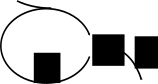
\includegraphics{cycle3.pdf}
\caption{A simple auto-catalytic cycle with extration of biomass reaction}
%\label{fig:autocatal}
\end{figure}
Biological systems are noisy by nature.
Thus, in order for metabolic pathways and cycles to be viable, they must be resistant to noise (meaning they should be able to perform their action, maintaining fluxes and concentrations, where necessary, even under perturbations).

We define a metabolic equilibrium state as a state where the concentrations of intermediate metabolites remains constant (excluding external input and output reactions, as defined by the topology of the network and problem at hand).
We will be investigating the number of equilibrium points, their respective concentrations and fluxes, and their stability.
By stability we refer to the ability of a network to converge back to the same equilibrium point in cases of small perturbations around it.

Mathematically we will be working in a vector space of the concentrations of the different metabolites, such that if there are two metabolites, $M_1$ and $M_2$, then $\vec{C}=(C_1,C_2)$ represents the state where $M_1$'s concentration is $C_1$ and $M_2$'s concentration is $C_2$.
If we now define a vectoric flux function, $\frac{d\vec{C}}{dt}=\vec{F}(\vec{C})$ (that is, a function that takes a vector of concentrations and returns the time derivative of each of the concentrations as a result of the implied network fluxes), we can formally define an equilibrium point, $\vec{C}^*$ as any point for which: $\vec{F}(\vec{C}^*)=0$.
Furthermore - dynamic theory states that such an equilibrium point will be stable iff the real parts of the eigenvalues of the Jacobian matrix of $\vec{F}()$ at $\vec{C}^*$ are all negative.

\section{Analyzing a simple cycle}
To warm up and get comfortable with the analysis method, we start with the simplest metabolic cycle possible, as is depicted in Figure \ref{simple-cycle}.
\begin{figure}[h]
\centering
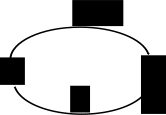
\includegraphics{cycle1.pdf}
\caption{A simple metabolic cycle}
\label{simple-cycle}
\end{figure}
For simplicity we will assume that $V_1$ is only a function of $C_1$, and $V_2$ is only a function of $C_2$.
Thus we get that:
\[\frac{d\vec{C}}{dt}=\vec{F}(C_1,C_2) = \bigg(
\begin{matrix}
    V_2(C_2)-V_1(C_1) \\
    V_1(C_1)-V_2(C_2)
\end{matrix}
\bigg)\]
Therefore an equilibrium point $\vec{C}^*$ must satisfy that: $\vec{F}(\vec{C}^*)=0$ implying that $V_1(C_1^*)=V_2(C_2^*)$.
In order to analyze stability we need to calculate the Jacobian matrix of $\vec{F}()$ which (once noting that $\frac{dV_1}{dC_2}=\frac{dV_2}{dC_1}=0$) becomes:
\[
J=\bigg(
\begin{matrix}
    -\frac{dV_1}{dC_1} & \frac{dV_2}{dC_2} \\
    \frac{dV_1}{dC_1} & -\frac{dV_2}{dC_2}
\end{matrix}
\bigg)
\]
If we use the notation of: $k_1=\frac{dV_1}{dC_1}$ and $k_2=\frac{dV_2}{dC_2}$, we can write the characteristic polynomial of the Jacobian matrix (the roots of which are its eigenvalues) as:
\[
\text{det}(\lambda I -J)=(\lambda+k_1)(\lambda+k_2)-k_1k_2=\lambda^2+(k_1+k_2)\lambda
\]
Which immediately indicates that the eigen values are $0$ and $-(k_1+k_2)$.
We can therefore conclude that no equilibrium point is stable, as all will have at least one non-negative eigenvalue.
However, if $k_1+k_2$ is positive, then the equilibrium point is semi-stable, in the sense that there is some direction (the direction corresponding to the eigen-vector with the $0$ eigenvalue) that is tangent to a line of equilibrium points (so small perturbations along this line will keep the system at equilibrium, but not the same equilibrium), and perturbations in the direction of the other eigenvector will return to the same equilibrium point.
Furthermore - as this setup, being a closed cycle, possesses the specific feature of conservation of mass (mathematically - $C_1+C_2$ is constant in time), and as each equilibrium point $\vec{C^*}$ can be characterized by such a total mass, if the perturbations do not change the total mass, the system will converge to the same equilibrium point, and if they do change the total mass, the system will converge to the unique equilibrium point defined for the modified mass.

As a sidenote, we coment that for Michaelis-Menten (MM) dynamics the derivatives are always positive, so that case results in all equilibrium points being semi-stable and conform to the analysis above.
\section{Analyzing a simple open cycle}
Once we got a little bit of a feel for the analysis of the dynamics of simple metabolic networks, we turn to a slightly more complicated case, as is depicted in Figure \ref{open-cycle}.
\begin{figure}[h]
\centering
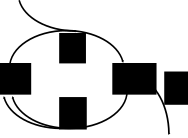
\includegraphics{cycle2.pdf}
\caption{A simple open metabolic cycle}
\label{open-cycle}
\end{figure}
Here the flux function is:
\[
\frac{d\vec{C}}{dt}=\vec{F}(\vec{C})=
\bigg(
\begin{matrix}
2V_2(C_2)-V_1(C_1) \\
V_1(C_1)-V_2(C_2)-V_3(C_2)
\end{matrix}
\bigg)
\]
Therefore equilibrium points must satisfy (for $C_1*$) that:
\[
2V_2(C_2^*)-V_1(C_1^*)=0 \rightarrow V_2(C_2^*)=V_1(C_1^*)/2
\]
and for $C_2^*$ (when substituting the above):
\[
V_1(C_1^*)-V_2(C_2^*)-V_3(C_2^*)=0 \rightarrow V_2(C_2^*)-V_3(C_2^*)=0 \rightarrow V_2(C_2^*)=V_3(C_2^*)
\]
So an equilibrium point must satisfy that:
\[ V_1(C_1^*)/2=V_2(C_2^*)=V_3(C_2^*) \]
For the current analysis we will consider two types of kinetics for $V_1$, $V_2$ and $V_3$: Linear and simple Michaelis-Menten.
We note that fluxes are alway zero when the substrate concentration is zero, implying that linear kinetics must be of the form $V(C)=aC$, and that the fluxes always increase when the substrate concentration increases, implying that the flux derivative w.r.t. its substrate is always positive.
Using the same notation as in the previous section for $k_1$, $k_2$ and $k_3$, we can write the Jacobian matrix of $V$ as:
\[
J=\bigg(
\begin{matrix}
    -k_1 & 2k_2 \\
    k_1 & -k_2-k_3
\end{matrix}
\bigg)
\]
and the characteristic polynomial is thus:
\[
\text{det}(\lambda I -J)=(\lambda+k_1)(\lambda+k_2+k_3)-2k_1k_2=\lambda^2+(k_1+k_2+k_3)\lambda -k_1k_2+k_1k_3
\]
The eigenvalues are therefore:
\[
\lambda_{1,2}=\frac{-(k_1+k_2+k_3)\pm \sqrt{(k_1+k_2+k_3)^2+4k_1k_2-4k_1k_3}}{2}
\]
Therefore, in order for the real part of both eigenvalues to be negative (the condition for a stable equilibrium point), $k_1+k_2+k_3$ must be positive (which always holds as $k_i>0$ for all $i$) and $4k_1k_2-4k_1k_3$ must be negative (implying that $k_3>k_2$, given that $k_1$ is positive).

We now turn to see what possible combinations of kinetics can satisfy these conditions:
\begin{itemize}
\item We note that the case of both $V_2$ and $V_3$ being linear (meaning that $V_2(C_2)=a_2C_2;V_3(C_2)=a_3C_2)$ is unprobable as it requires that $a_2=a_3$ in order for an equilibrium point to exist.
\item If $V_2$ is linear and $V_3$ is MM, then they must intersect at an equilibrium point.
They intersect at the trivial point where $C_2=0$.
As MM is a concave function, if they intersect at a larger concentration point, then at the point of intersection $k_3$ will be smaller than $a_2=k_2$ making that point unstable.
\end{itemize}
We therefore conclude that $V_2$ cannot be linear but rather must be MM, and that $V_1$ and $V_3$ can be either linear or MM.

As at an equilibrium point $V_2(C_2^*)=V_3(C_2^*)$, and as we are restricted to linear or MM kinetics, it follows that there is at most only one concentration $C_2$ (other than $C_2=0$) for which this condition holds.
For this concentration, if there exists a concentration $C_1$ that satisfies $V_1(C_1)/2=V_2(C_2)$ then there exists an equilibrium point for the metabolic network.
At these concentrations, if $k_3>k_2$ (as is always the case for linear $V_3$, and is sometimes the case for MM $k_2,k_3$, which we will analyze below), then the equilibrium point is stable.

To get some intuition on how stability works, if we assume that the system is in the equilibrium state, and then somehow a small deviation in the concentrations occure - then there are two possibilities: either the total number of carbons in the cycle ($C_1+C_2$) increased, or it decreased.
If it increased - then at some point $C_2$'s concentration will be above the equilibrium point.
At this point - as $k_3>k_2$, more carbons will be taken out of the cycle via $V_3$ than recycled via $V_2$, thus decreasing the total number of carbons in the cycle.
If, on the other hand, the total number of carbons in the cycle is somewhat smaller than the number at the equilibrium state, then at some point $C_2$ will be smaller than its value at the equilibrium point, resulting in $V_2>V_3$.
At this point, the flux of carbons out of the cycle is smaller than the flux of carbons that are recycled in the cycle.
As new carbons are being added to the cycle via $V_1$, the total number of carbons in the cycle will increase.

\subsection{Analyzing intersection points of MM kinetics and linear kinetics}
The general form of a MM kinetics equation is:
\[
V(C)=\frac{V_{max}C}{K_m+C}
\]
Therefore, it intersects a straight line of the form $V(C)=aC$ at the solutions to the equation:
\[
aC=\frac{V_{max}C}{K_m+C} \rightarrow aC^2+C(aK_m-V_{max})
\]
that is, at $C=0$ and $C=V_{max}-aK_m$
In order for the non-trivial solution to be feasible we must therefore require that $V_{max}>aK_m$.

In the case of two MM kinetics fluxes:
\[
V_a(C)=\frac{V_{a,max}C}{K_{a,m}+C};
V_b(C)=\frac{V_{b,max}C}{K_{b,m}+C}
\]
The intersection points are the solutions to the equation:
\[
\frac{V_{a,max}C}{K_{a,m}+C}=\frac{V_{b,max}C}{K_{b,m}+C} \rightarrow (V_{a,max}C)(K_{b,m}+C)=(V_{b,max}C)(K_{a,m}+C)
\]
Which are at $C=0$ and at:
\[
C(V_{a,max}-V_{b,max})=V_{b,max}K_{a,m}-V_{a,max}K_{b,m} \rightarrow C=\frac{V_{b,max}K_{a,m}-V_{a,max}K_{b,m}}{V_{a,max}-V_{b,max}}
\]
Requiring a positive intersection and assuming w.l.o.g. that $V_{a,max}>V_{b,max}$ thus gives:
\[
V_{b,max}K_{a,m}-V_{a,max}K_{b,m}>0 \rightarrow V_{b,max}K_{a,m}>V_{a,max}K_{b,m}
\]
concluding that:
\[
\frac{V_{b,max}}{V_{a,max}}>\frac{K_{b,m}}{K_{a,m}}
\]
Integrating this result with the stability requirement (that at the intersection point $k_3>k_2$), noting that this implies that $V_{3,max}>V_{2,max}$ we must therefore assign $a \rightarrow 3$ and $b \rightarrow 2$ to get:
\[
\frac{V_{2,max}}{V_{3,max}}>\frac{K_{2,m}}{K_{3,m}}
\]
as the requirement on the kinetic parameters of $V_2()$ and $V_3()$.

TODO: add analysis of convergence via analytical solution to linear differential equations.
analyze cases of substrate inhibition.
\end{document}
